\documentclass[../main.tex]{subfiles}

\begin{document}
Like many other fields dealing with the classification of images, the DNN revolution impacted Facial Expression Recognition (FER).
This field can benefit from both major DNN architectures. The CNN - enabling a better understanding of image data through learned features.
The RNN - enabling a better understanding of temporal relationships in time series data.
In this section, we review a few studies in the field that we feel best suit our project's goals.
\par

A recent study in the field \cite{emotionnet-nano} attempted to create a very efficient model that would be able
to recognize facial expression while running on an embedded device.  EmotionNet Nano, the model introduced in the paper,
was constructed with a similar philosophy to \cite{effnet}. The authors started with a base model and then defined an
optimization problem to maximize the model's accuracy while constraining it to a size of less than 1M parameters.
As described in the paper, the use of automatic network design exploration provided a significant advantage over hand-crafted
designs in its ability to produce very heterogeneous blocks that better fit the problem.
As we can see from the model architecture \ref{fig:emotionnet_nano}, two fascinating phenomena exist in this model:

\begin{itemize}
    \item We can see that the layers' shapes differ from one to another, increasing and decreasing the number of filters through the network.
    \item The residual connections are not the same for each layer and even skip some layers entirely.
        This phenomenon is referred to in the paper as selective long-range connectivity. The model generator's ability to choose such
        specific residual connections creates a healthy balance between model expressiveness and ease of training.
    \item Maybe most interesting are the 1x1 convolution layers that tale outputs from multiple 3x3 convulsions
        and connect back to the network at deeper layers. These connections provide dimensionality reductions and retain older
        features by mixing the channels, meaning the model's expressiveness is increased for a low computational cost.
\end{itemize}

We chose to focus on this paper because of the model's simplicity combined with its state of the art performance. In the paper,
the authors present two models. One smaller and less accurate model, achieving 92\% accuracy on CK+,
and the other slightly bigger achieving 97\% accuracy on CK+. The "Big" model only has ~200k parameters, meaning it would be effortless to
train and experiment with it. The other reason is its performance. Though the authors optimized the model for inference performance,
its size means that it will be relatively light to train, which is vital for our use case of perpetual training personalized model.
We will discuss our experiments in more depth in the experiments section, though this model will allow us to retrain it on different data
with different labels and even make adjustments to the model quickly, which is also very important to us.
\par

\begin{figure}[htp]
    \centering
    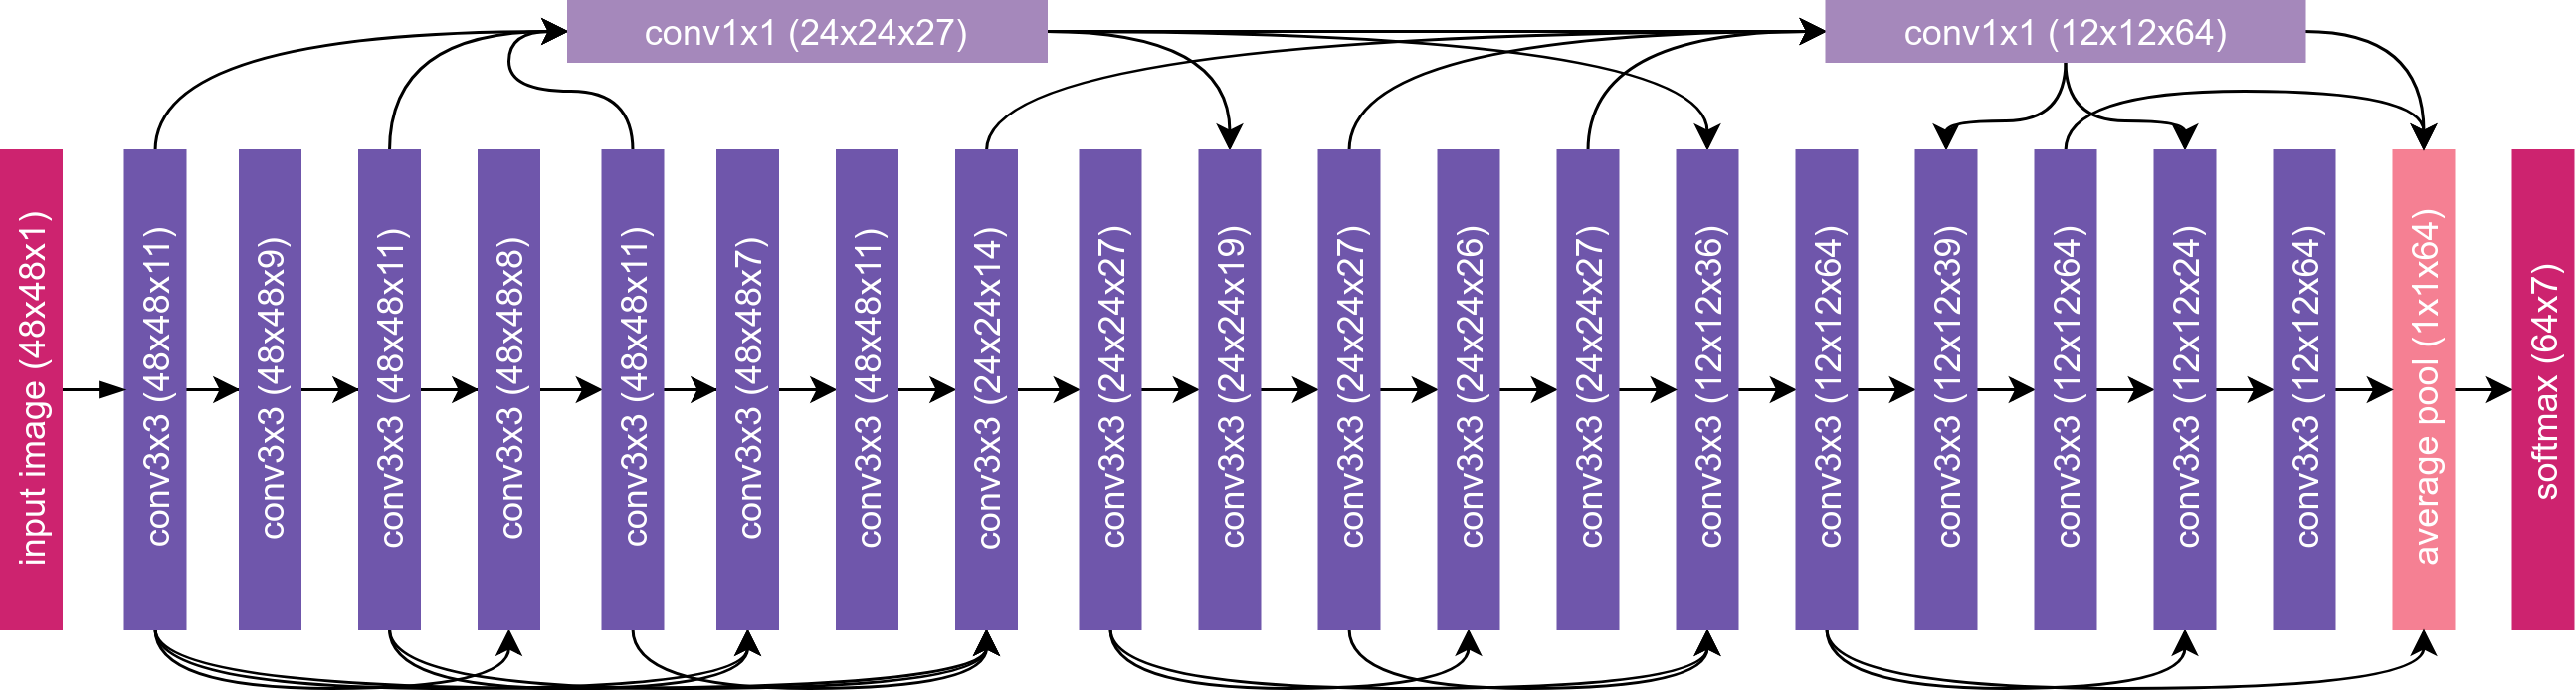
\includegraphics[width=12cm]{figures/emotionnet_nano.png}   
    \caption{EmotionNet Nano architecture as as shown in the paper \cite{emotionnet-nano}}
    \label{fig:emotionnet_nano} 
\end{figure}


\end{document}